\section{Implementation}

\subsection{Crossfire Firefox Extension}
The first implementation of the Crossfire protocol is an extension implements
the protocol as an extension to Firefox and Firebug. The extension is
implemented entirely in JavaScript, using a modular design to allow us to share
code between client and server implementations, as well as cross-browser
implementations. This extension implements a flexible transport layer, allowing
the extension to operate as either a Crossfire client or server. This will also
enable both client and server to be implemented on top of other transport
layers, such as Web Sockets or HTTP.

The extension can be started in client or server mode either from the Firefox
user interface, or via command-line switches to Firefox. This latter mode of
operation allows external tools to launch Firefox and start the Crossfire server
listening on a known port so that the external tool may automatically connect
back to it. Figure \ref{fig:crossfire-arch}

In order to support Firebug's ability to operate both in-process and
out-of-process, an asynchronous API which we called BrowserToolsInterface was
put in place to broker calls between Firebug's front- and back-end pieces.

\subsection{Crossfire Tools API}
The Crossfire extension also implements an API, called the ``Crossfire Tools
API'' which enables extensibility of the Crossfire system and protocol. Firebug
features such as the Console, Inspector, and Net Panel, are implemented as tools
using the API, allowing them to be enabled/disabled independently.

A tool can be implemented as a JavaScript file or collection of files that
implements the Crossfire Tools API. The tool registers itself with the core
Crossfire Module, providing an identification string that is used to identify
messages via the 'tool' header. In server operation, the tool is then able to
receive notification when a connection is created or when request packets are
received. The Tools API allows a tool to access Crossfire's transport layer in
order to send events or command responses.  Typically, a tool operating within
the context of a Crossfire server might register listeners with one or more
Firebug modules, in order to dispatch events generated by the module to the
remote connection. A tool operating as part of a Crossfire client would process
the events sent from the server tool, and update part of the client UI, such as
a Firebug panel. The tool could also listen for client events from the UI, and
send the appropriate requests to the server, to be handled by the tool's
server-side component.

\begin{figure}[htp]
  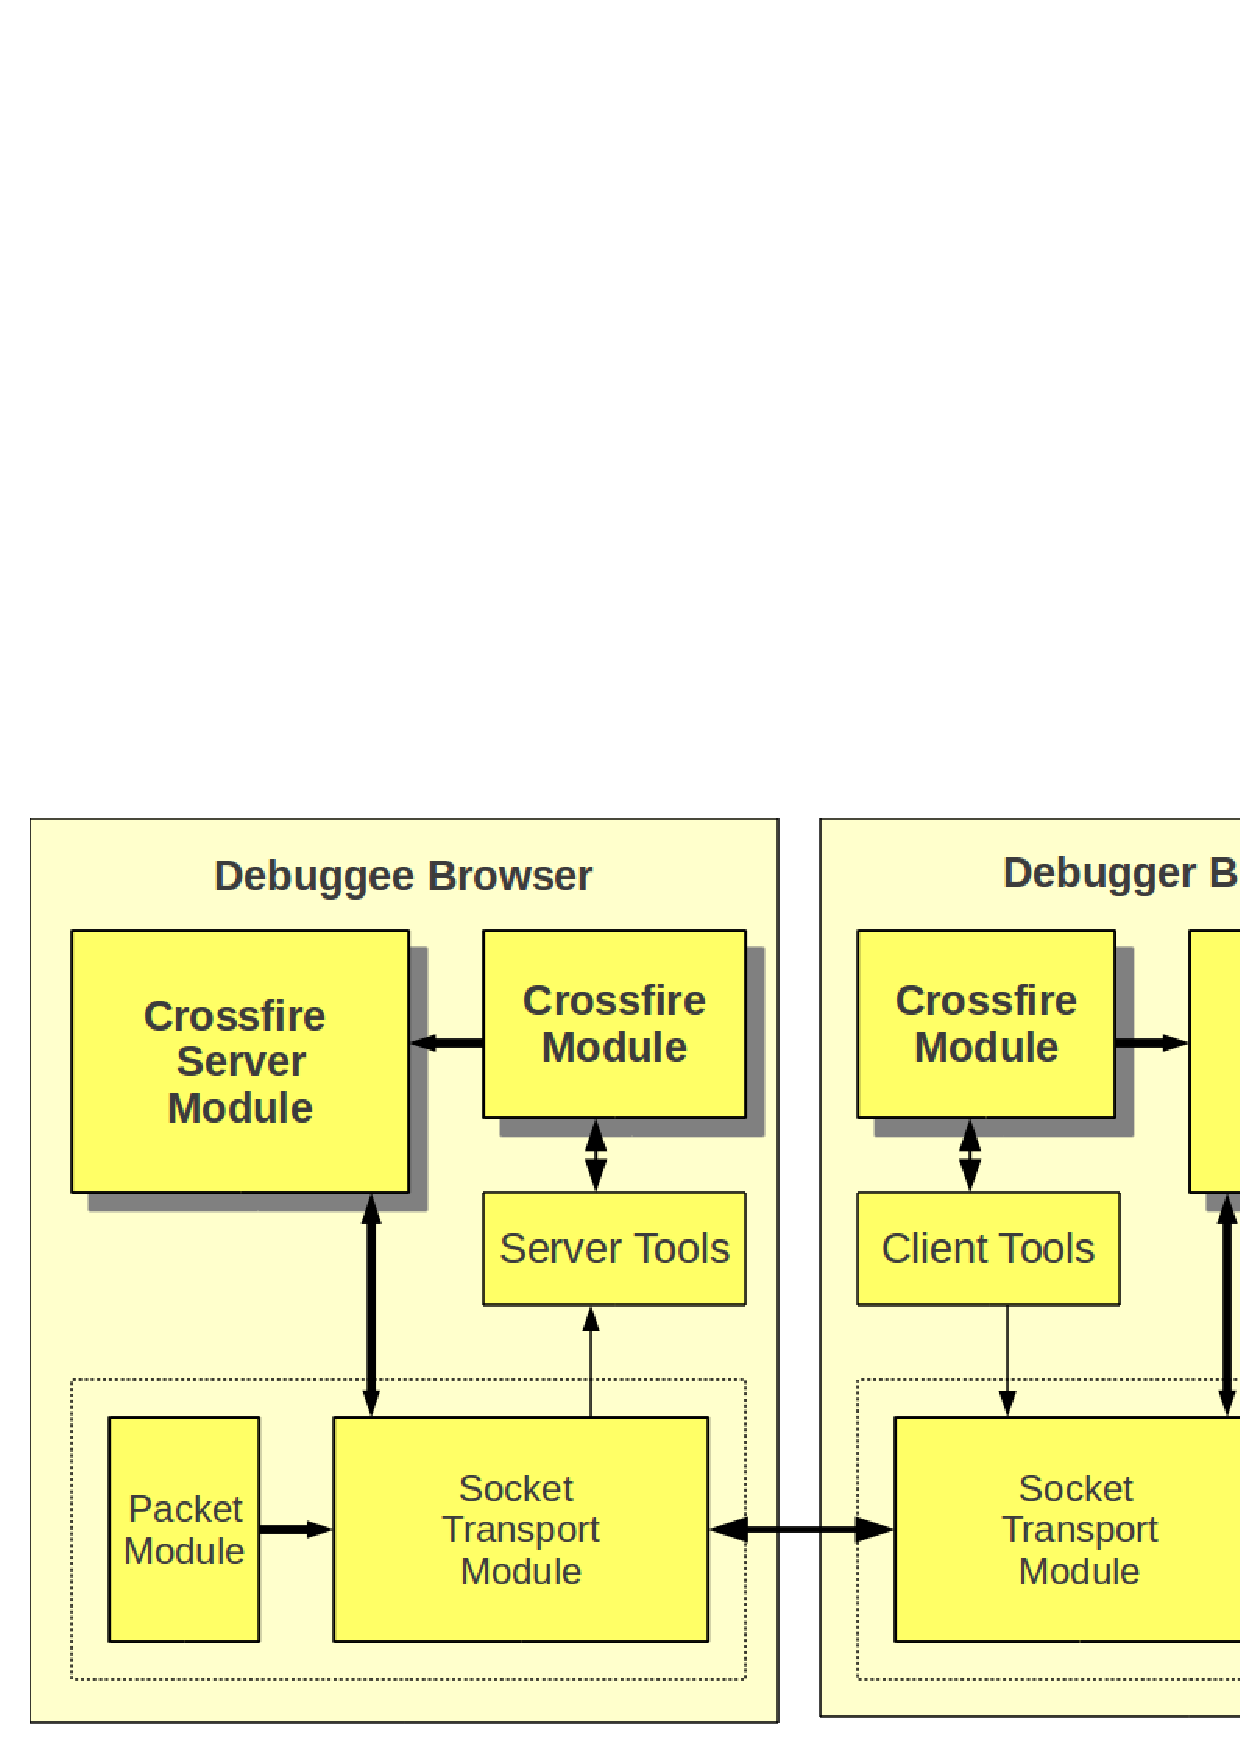
\includegraphics  [width = 86 mm] {figures/crossfire-arch4.png}
  \caption{Crossfire Firefox Extension Architecture}
 \label{fig:crossfire-arch}
\end{figure}

\subsection{Modules}

\subsection {Browser Tools Interface}